%%%%%%%%%%%%%%%%%%%%%%%%%%%%%%%%%%%%%%%%%
% Libro Programación FP: guía de supervivencia
% Luis del Moral Martínez
%
% Licencia:
% CC BY-NC-SA 4.0 https:(//creativecommons.org/licenses/by-nc-sa/4.0/)
%
% Este documento usa la plantilla 'The Legrand Orange Book', version 2.4 (26/09/2018)
% La plantilla fue descargada de http://www.LaTeXTemplates.com
%
% Autor original de la plantilla:
% Mathias Legrand (legrand.mathias@gmail.com) con modificaciones realizadas por:
% Vel (vel@latextemplates.com)
%
% Licencia original de la plantilla:
% CC BY-NC-SA 3.0 (http://creativecommons.org/licenses/by-nc-sa/3.0/)
% (DAW y DAM)
%
% Nota importante:
% Las imágenes de cabecera de los capítulos deben tener una relación de aspecto de 2:1 (anchura:altura)
% ejemplo: 920px x 460px (anchura x altura).
%
%%%%%%%%%%%%%%%%%%%%%%%%%%%%%%%%%%%%%%%%%

%----------------------------------------------------------------------------------------
%	PAQUETES Y CONFIGURACIÓN DEL DOCUMENTO
%----------------------------------------------------------------------------------------

\documentclass[12pt,fleqn]{book} % Fuente por defecto y ecuaciones alineadas a la izquierda

%%%%%%%%%%%%%%%%%%%%%%%%%%%%%%%%%%%%%%%%%
% Libro Programación FP: guía de supervivencia
% Luis del Moral Martínez
% Estructura del proyecto
%
% Licencia:
% CC BY-NC-SA 4.0 https:(//creativecommons.org/licenses/by-nc-sa/4.0/)
%
% Este documento usa la plantilla The Legrand Orange Book, version 2.4 (26/09/2018)
% La plantilla fue descargada de http://www.LaTeXTemplates.com
%
% Autor original de la plantilla:
% Mathias Legrand (legrand.mathias@gmail.com) con modificaciones realizadas por:
% Vel (vel@latextemplates.com)
%
% Licencia original de la plantilla:
% CC BY-NC-SA 3.0 (http://creativecommons.org/licenses/by-nc-sa/3.0/)
%
%%%%%%%%%%%%%%%%%%%%%%%%%%%%%%%%%%%%%%%%%

%----------------------------------------------------------------------------------------
%	VARIOUS REQUIRED PACKAGES AND CONFIGURATIONS
%----------------------------------------------------------------------------------------

\usepackage{graphicx} % Required for including pictures
\graphicspath{{Pictures/}} % Specifies the directory where pictures are stored

\usepackage{lipsum} % Inserts dummy text

\usepackage{tikz} % Required for drawing custom shapes

\usepackage[spanish]{babel} % Spanish language/hyphenation

\usepackage{enumitem} % Customize lists
\setlist{nolistsep} % Reduce spacing between bullet points and numbered lists

\usepackage{booktabs} % Required for nicer horizontal rules in tables

\usepackage{xcolor} % Required for specifying colors by name
\definecolor{ocre}{RGB}{243,102,25} % Define the orange color used for highlighting throughout the book

%----------------------------------------------------------------------------------------
%	MARGINS
%----------------------------------------------------------------------------------------

\usepackage{geometry} % Required for adjusting page dimensions and margins

\geometry{
	paper=a4paper, % Paper size, change to letterpaper for US letter size
	top=3cm, % Top margin
	bottom=3cm, % Bottom margin
	left=3cm, % Left margin
	right=3cm, % Right margin
	headheight=14pt, % Header height
	footskip=1.4cm, % Space from the bottom margin to the baseline of the footer
	headsep=10pt, % Space from the top margin to the baseline of the header
	%showframe, % Uncomment to show how the type block is set on the page
}

%----------------------------------------------------------------------------------------
%	FONTS
%----------------------------------------------------------------------------------------

\usepackage{avant} % Use the Avantgarde font for headings
%\usepackage{times} % Use the Times font for headings
\usepackage{mathptmx} % Use the Adobe Times Roman as the default text font together with math symbols from the Sym­bol, Chancery and Com­puter Modern fonts

\usepackage{microtype} % Slightly tweak font spacing for aesthetics
\usepackage[utf8]{inputenc} % Required for including letters with accents
\usepackage[T1]{fontenc} % Use 8-bit encoding that has 256 glyphs

%----------------------------------------------------------------------------------------
%	BIBLIOGRAPHY AND INDEX
%----------------------------------------------------------------------------------------

\usepackage[style=numeric,citestyle=numeric,sorting=nyt,sortcites=true,autopunct=true,babel=hyphen,hyperref=true,abbreviate=false,backref=true,backend=biber]{biblatex}
\addbibresource{bibliography.bib} % BibTeX bibliography file
\defbibheading{bibempty}{}

\usepackage{calc} % For simpler calculation - used for spacing the index letter headings correctly
\usepackage{makeidx} % Required to make an index
\makeindex % Tells LaTeX to create the files required for indexing

%----------------------------------------------------------------------------------------
%	MAIN TABLE OF CONTENTS
%----------------------------------------------------------------------------------------

\usepackage{titletoc} % Required for manipulating the table of contents

\contentsmargin{0cm} % Removes the default margin

% Part text styling (this is mostly taken care of in the PART HEADINGS section of this file)
\titlecontents{part}
	[0cm] % Left indentation
	{\addvspace{20pt}\bfseries} % Spacing and font options for parts
	{}
	{}
	{}

% Chapter text styling
\titlecontents{chapter}
	[1.25cm] % Left indentation
	{\addvspace{12pt}\large\sffamily\bfseries} % Spacing and font options for chapters
	{\color{ocre!60}\contentslabel[\Large\thecontentslabel]{1.25cm}\color{ocre}} % Formatting of numbered sections of this type
	{\color{ocre}} % Formatting of numberless sections of this type
	{\color{ocre!60}\normalsize\;\titlerule*[.5pc]{.}\;\thecontentspage} % Formatting of the filler to the right of the heading and the page number

% Section text styling
\titlecontents{section}
	[1.25cm] % Left indentation
	{\addvspace{3pt}\sffamily\bfseries} % Spacing and font options for sections
	{\contentslabel[\thecontentslabel]{1.25cm}} % Formatting of numbered sections of this type
	{} % Formatting of numberless sections of this type
	{\hfill\color{black}\thecontentspage} % Formatting of the filler to the right of the heading and the page number

% Subsection text styling
\titlecontents{subsection}
	[1.25cm] % Left indentation
	{\addvspace{1pt}\sffamily\small} % Spacing and font options for subsections
	{\contentslabel[\thecontentslabel]{1.25cm}} % Formatting of numbered sections of this type
	{} % Formatting of numberless sections of this type
	{\ \titlerule*[.5pc]{.}\;\thecontentspage} % Formatting of the filler to the right of the heading and the page number

% Figure text styling
\titlecontents{figure}
	[1.25cm] % Left indentation
	{\addvspace{1pt}\sffamily\small} % Spacing and font options for figures
	{\thecontentslabel\hspace*{1em}} % Formatting of numbered sections of this type
	{} % Formatting of numberless sections of this type
	{\ \titlerule*[.5pc]{.}\;\thecontentspage} % Formatting of the filler to the right of the heading and the page number

% Table text styling
\titlecontents{table}
	[1.25cm] % Left indentation
	{\addvspace{1pt}\sffamily\small} % Spacing and font options for tables
	{\thecontentslabel\hspace*{1em}} % Formatting of numbered sections of this type
	{} % Formatting of numberless sections of this type
	{\ \titlerule*[.5pc]{.}\;\thecontentspage} % Formatting of the filler to the right of the heading and the page number

%----------------------------------------------------------------------------------------
%	MINI TABLE OF CONTENTS IN PART HEADS
%----------------------------------------------------------------------------------------

% Chapter text styling
\titlecontents{lchapter}
	[0em] % Left indentation
	{\addvspace{15pt}\large\sffamily\bfseries} % Spacing and font options for chapters
	{\color{ocre}\contentslabel[\Large\thecontentslabel]{1.25cm}\color{ocre}} % Chapter number
	{}  
	{\color{ocre}\normalsize\sffamily\bfseries\;\titlerule*[.5pc]{.}\;\thecontentspage} % Page number

% Section text styling
\titlecontents{lsection}
	[0em] % Left indentation
	{\sffamily\small} % Spacing and font options for sections
	{\contentslabel[\thecontentslabel]{1.25cm}} % Section number
	{}
	{}

% Subsection text styling (note these aren't shown by default, display them by searchings this file for tocdepth and reading the commented text)
\titlecontents{lsubsection}
	[.5em] % Left indentation
	{\sffamily\footnotesize} % Spacing and font options for subsections
	{\contentslabel[\thecontentslabel]{1.25cm}}
	{}
	{}

%----------------------------------------------------------------------------------------
%	HEADERS AND FOOTERS
%----------------------------------------------------------------------------------------

\usepackage{fancyhdr} % Required for header and footer configuration

\pagestyle{fancy} % Enable the custom headers and footers

\renewcommand{\chaptermark}[1]{\markboth{\sffamily\normalsize\bfseries\chaptername\ \thechapter.\ #1}{}} % Styling for the current chapter in the header
\renewcommand{\sectionmark}[1]{\markright{\sffamily\normalsize\thesection\hspace{5pt}#1}{}} % Styling for the current section in the header

\fancyhf{} % Clear default headers and footers
\fancyhead[LE,RO]{\sffamily\normalsize\thepage} % Styling for the page number in the header
\fancyhead[LO]{\rightmark} % Print the nearest section name on the left side of odd pages
\fancyhead[RE]{\leftmark} % Print the current chapter name on the right side of even pages
%\fancyfoot[C]{\thepage} % Uncomment to include a footer

\renewcommand{\headrulewidth}{0.5pt} % Thickness of the rule under the header

\fancypagestyle{plain}{% Style for when a plain pagestyle is specified
	\fancyhead{}\renewcommand{\headrulewidth}{0pt}%
}

% Removes the header from odd empty pages at the end of chapters
\makeatletter
\renewcommand{\cleardoublepage}{
\clearpage\ifodd\c@page\else
\hbox{}
\vspace*{\fill}
\thispagestyle{empty}
\newpage
\fi}

%----------------------------------------------------------------------------------------
%	THEOREM STYLES
%----------------------------------------------------------------------------------------

\usepackage{amsmath,amsfonts,amssymb,amsthm} % For math equations, theorems, symbols, etc

\newcommand{\intoo}[2]{\mathopen{]}#1\,;#2\mathclose{[}}
\newcommand{\ud}{\mathop{\mathrm{{}d}}\mathopen{}}
\newcommand{\intff}[2]{\mathopen{[}#1\,;#2\mathclose{]}}
\renewcommand{\qedsymbol}{$\blacksquare$}
\newtheorem{notation}{Notation}[chapter]

% Boxed/framed environments
\newtheoremstyle{ocrenumbox}% Theorem style name
{0pt}% Space above
{0pt}% Space below
{\normalfont}% Body font
{}% Indent amount
{\small\bf\sffamily\color{ocre}}% Theorem head font
{\;}% Punctuation after theorem head
{0.25em}% Space after theorem head
{\small\sffamily\color{ocre}\thmname{#1}\nobreakspace\thmnumber{\@ifnotempty{#1}{}\@upn{#2}}% Theorem text (e.g. Theorem 2.1)
\thmnote{\nobreakspace\the\thm@notefont\sffamily\bfseries\color{black}---\nobreakspace#3.}} % Optional theorem note

\newtheoremstyle{blacknumex}% Theorem style name
{5pt}% Space above
{5pt}% Space below
{\normalfont}% Body font
{} % Indent amount
{\small\bf\sffamily}% Theorem head font
{\;}% Punctuation after theorem head
{0.25em}% Space after theorem head
{\small\sffamily{\tiny\ensuremath{\blacksquare}}\nobreakspace\thmname{#1}\nobreakspace\thmnumber{\@ifnotempty{#1}{}\@upn{#2}}% Theorem text (e.g. Theorem 2.1)
\thmnote{\nobreakspace\the\thm@notefont\sffamily\bfseries---\nobreakspace#3.}}% Optional theorem note

\newtheoremstyle{blacknumbox} % Theorem style name
{0pt}% Space above
{0pt}% Space below
{\normalfont}% Body font
{}% Indent amount
{\small\bf\sffamily}% Theorem head font
{\;}% Punctuation after theorem head
{0.25em}% Space after theorem head
{\small\sffamily\thmname{#1}\nobreakspace\thmnumber{\@ifnotempty{#1}{}\@upn{#2}}% Theorem text (e.g. Theorem 2.1)
\thmnote{\nobreakspace\the\thm@notefont\sffamily\bfseries---\nobreakspace#3.}}% Optional theorem note

% Non-boxed/non-framed environments
\newtheoremstyle{ocrenum}% Theorem style name
{5pt}% Space above
{5pt}% Space below
{\normalfont}% Body font
{}% Indent amount
{\small\bf\sffamily\color{ocre}}% Theorem head font
{\;}% Punctuation after theorem head
{0.25em}% Space after theorem head
{\small\sffamily\color{ocre}\thmname{#1}\nobreakspace\thmnumber{\@ifnotempty{#1}{}\@upn{#2}}% Theorem text (e.g. Theorem 2.1)
\thmnote{\nobreakspace\the\thm@notefont\sffamily\bfseries\color{black}---\nobreakspace#3.}} % Optional theorem note
\makeatother

% Defines the theorem text style for each type of theorem to one of the three styles above
\newcounter{dummy} 
\numberwithin{dummy}{section}
\theoremstyle{ocrenumbox}
\newtheorem{theoremeT}[dummy]{Theorem}
\newtheorem{problem}{Problem}[chapter]
\newtheorem{exerciseT}{Exercise}[chapter]
\theoremstyle{blacknumex}
\newtheorem{exampleT}{Example}[chapter]
\theoremstyle{blacknumbox}
\newtheorem{vocabulary}{Vocabulary}[chapter]
\newtheorem{definitionT}{Definition}[section]
\newtheorem{corollaryT}[dummy]{Corollary}
\theoremstyle{ocrenum}
\newtheorem{proposition}[dummy]{Proposition}

%----------------------------------------------------------------------------------------
%	DEFINITION OF COLORED BOXES
%----------------------------------------------------------------------------------------

\RequirePackage[framemethod=default]{mdframed} % Required for creating the theorem, definition, exercise and corollary boxes

% Theorem box
\newmdenv[skipabove=7pt,
skipbelow=7pt,
backgroundcolor=black!5,
linecolor=ocre,
innerleftmargin=5pt,
innerrightmargin=5pt,
innertopmargin=5pt,
leftmargin=0cm,
rightmargin=0cm,
innerbottommargin=5pt]{tBox}

% Exercise box	  
\newmdenv[skipabove=7pt,
skipbelow=7pt,
rightline=false,
leftline=true,
topline=false,
bottomline=false,
backgroundcolor=ocre!10,
linecolor=ocre,
innerleftmargin=5pt,
innerrightmargin=5pt,
innertopmargin=5pt,
innerbottommargin=5pt,
leftmargin=0cm,
rightmargin=0cm,
linewidth=4pt]{eBox}	

% Definition box
\newmdenv[skipabove=7pt,
skipbelow=7pt,
rightline=false,
leftline=true,
topline=false,
bottomline=false,
linecolor=ocre,
innerleftmargin=5pt,
innerrightmargin=5pt,
innertopmargin=0pt,
leftmargin=0cm,
rightmargin=0cm,
linewidth=4pt,
innerbottommargin=0pt]{dBox}	

% Corollary box
\newmdenv[skipabove=7pt,
skipbelow=7pt,
rightline=false,
leftline=true,
topline=false,
bottomline=false,
linecolor=gray,
backgroundcolor=black!5,
innerleftmargin=5pt,
innerrightmargin=5pt,
innertopmargin=5pt,
leftmargin=0cm,
rightmargin=0cm,
linewidth=4pt,
innerbottommargin=5pt]{cBox}

% Creates an environment for each type of theorem and assigns it a theorem text style from the "Theorem Styles" section above and a colored box from above
\newenvironment{theorem}{\begin{tBox}\begin{theoremeT}}{\end{theoremeT}\end{tBox}}
\newenvironment{exercise}{\begin{eBox}\begin{exerciseT}}{\hfill{\color{ocre}\tiny\ensuremath{\blacksquare}}\end{exerciseT}\end{eBox}}				  
\newenvironment{definition}{\begin{dBox}\begin{definitionT}}{\end{definitionT}\end{dBox}}	
\newenvironment{example}{\begin{exampleT}}{\hfill{\tiny\ensuremath{\blacksquare}}\end{exampleT}}		
\newenvironment{corollary}{\begin{cBox}\begin{corollaryT}}{\end{corollaryT}\end{cBox}}	

%----------------------------------------------------------------------------------------
%	REMARK ENVIRONMENT
%----------------------------------------------------------------------------------------

\newenvironment{remark}{\par\vspace{10pt}\small % Vertical white space above the remark and smaller font size
\begin{list}{}{
\leftmargin=35pt % Indentation on the left
\rightmargin=25pt}\item\ignorespaces % Indentation on the right
\makebox[-2.5pt]{\begin{tikzpicture}[overlay]
\node[draw=ocre!60,line width=1pt,circle,fill=ocre!25,font=\sffamily\bfseries,inner sep=2pt,outer sep=0pt] at (-15pt,0pt){\textcolor{ocre}{R}};\end{tikzpicture}} % Orange R in a circle
\advance\baselineskip -1pt}{\end{list}\vskip5pt} % Tighter line spacing and white space after remark

%----------------------------------------------------------------------------------------
%	SECTION NUMBERING IN THE MARGIN
%----------------------------------------------------------------------------------------

\makeatletter
\renewcommand{\@seccntformat}[1]{\llap{\textcolor{ocre}{\csname the#1\endcsname}\hspace{1em}}}                    
\renewcommand{\section}{\@startsection{section}{1}{\z@}
{-4ex \@plus -1ex \@minus -.4ex}
{1ex \@plus.2ex }
{\normalfont\large\sffamily\bfseries}}
\renewcommand{\subsection}{\@startsection {subsection}{2}{\z@}
{-3ex \@plus -0.1ex \@minus -.4ex}
{0.5ex \@plus.2ex }
{\normalfont\sffamily\bfseries}}
\renewcommand{\subsubsection}{\@startsection {subsubsection}{3}{\z@}
{-2ex \@plus -0.1ex \@minus -.2ex}
{.2ex \@plus.2ex }
{\normalfont\small\sffamily\bfseries}}                        
\renewcommand\paragraph{\@startsection{paragraph}{4}{\z@}
{-2ex \@plus-.2ex \@minus .2ex}
{.1ex}
{\normalfont\small\sffamily\bfseries}}

%----------------------------------------------------------------------------------------
%	PART HEADINGS
%----------------------------------------------------------------------------------------

% Numbered part in the table of contents
\newcommand{\@mypartnumtocformat}[2]{%
	\setlength\fboxsep{0pt}%
	\noindent\colorbox{ocre!20}{\strut\parbox[c][.7cm]{\ecart}{\color{ocre!70}\Large\sffamily\bfseries\centering#1}}\hskip\esp\colorbox{ocre!40}{\strut\parbox[c][.7cm]{\linewidth-\ecart-\esp}{\Large\sffamily\centering#2}}%
}

% Unnumbered part in the table of contents
\newcommand{\@myparttocformat}[1]{%
	\setlength\fboxsep{0pt}%
	\noindent\colorbox{ocre!40}{\strut\parbox[c][.7cm]{\linewidth}{\Large\sffamily\centering#1}}%
}

\newlength\esp
\setlength\esp{4pt}
\newlength\ecart
\setlength\ecart{1.2cm-\esp}
\newcommand{\thepartimage}{}%
\newcommand{\partimage}[1]{\renewcommand{\thepartimage}{#1}}%
\def\@part[#1]#2{%
\ifnum \c@secnumdepth >-2\relax%
\refstepcounter{part}%
\addcontentsline{toc}{part}{\texorpdfstring{\protect\@mypartnumtocformat{\thepart}{#1}}{\partname~\thepart\ ---\ #1}}
\else%
\addcontentsline{toc}{part}{\texorpdfstring{\protect\@myparttocformat{#1}}{#1}}%
\fi%
\startcontents%
\markboth{}{}%
{\thispagestyle{empty}%
\begin{tikzpicture}[remember picture,overlay]%
\node at (current page.north west){\begin{tikzpicture}[remember picture,overlay]%	
\fill[ocre!20](0cm,0cm) rectangle (\paperwidth,-\paperheight);
\node[anchor=north] at (4cm,-3.25cm){\color{ocre!40}\fontsize{220}{100}\sffamily\bfseries\thepart}; 
\node[anchor=south east] at (\paperwidth-1cm,-\paperheight+1cm){\parbox[t][][t]{8.5cm}{
\printcontents{l}{0}{\setcounter{tocdepth}{1}}% The depth to which the Part mini table of contents displays headings; 0 for chapters only, 1 for chapters and sections and 2 for chapters, sections and subsections
}};
\node[anchor=north east] at (\paperwidth-1.5cm,-3.25cm){\parbox[t][][t]{15cm}{\strut\raggedleft\color{white}\fontsize{30}{30}\sffamily\bfseries#2}};
\end{tikzpicture}};
\end{tikzpicture}}%
\@endpart}
\def\@spart#1{%
\startcontents%
\phantomsection
{\thispagestyle{empty}%
\begin{tikzpicture}[remember picture,overlay]%
\node at (current page.north west){\begin{tikzpicture}[remember picture,overlay]%	
\fill[ocre!20](0cm,0cm) rectangle (\paperwidth,-\paperheight);
\node[anchor=north east] at (\paperwidth-1.5cm,-3.25cm){\parbox[t][][t]{15cm}{\strut\raggedleft\color{white}\fontsize{30}{30}\sffamily\bfseries#1}};
\end{tikzpicture}};
\end{tikzpicture}}
\addcontentsline{toc}{part}{\texorpdfstring{%
\setlength\fboxsep{0pt}%
\noindent\protect\colorbox{ocre!40}{\strut\protect\parbox[c][.7cm]{\linewidth}{\Large\sffamily\protect\centering #1\quad\mbox{}}}}{#1}}%
\@endpart}
\def\@endpart{\vfil\newpage
\if@twoside
\if@openright
\null
\thispagestyle{empty}%
\newpage
\fi
\fi
\if@tempswa
\twocolumn
\fi}

%----------------------------------------------------------------------------------------
%	CHAPTER HEADINGS
%----------------------------------------------------------------------------------------

% A switch to conditionally include a picture, implemented by Christian Hupfer
\newif\ifusechapterimage
\usechapterimagetrue
\newcommand{\thechapterimage}{}%
\newcommand{\chapterimage}[1]{\ifusechapterimage\renewcommand{\thechapterimage}{#1}\fi}%
\newcommand{\autodot}{.}
\def\@makechapterhead#1{%
{\parindent \z@ \raggedright \normalfont
\ifnum \c@secnumdepth >\m@ne
\if@mainmatter
\begin{tikzpicture}[remember picture,overlay]
\node at (current page.north west)
{\begin{tikzpicture}[remember picture,overlay]
\node[anchor=north west,inner sep=0pt] at (0,0) {\ifusechapterimage\includegraphics[width=\paperwidth]{\thechapterimage}\fi};
\draw[anchor=west] (\Gm@lmargin,-9cm) node [line width=2pt,rounded corners=15pt,draw=ocre,fill=white,fill opacity=0.5,inner sep=15pt]{\strut\makebox[22cm]{}};
\draw[anchor=west] (\Gm@lmargin+.3cm,-9cm) node {\huge\sffamily\bfseries\color{black}\thechapter\autodot~#1\strut};
\end{tikzpicture}};
\end{tikzpicture}
\else
\begin{tikzpicture}[remember picture,overlay]
\node at (current page.north west)
{\begin{tikzpicture}[remember picture,overlay]
\node[anchor=north west,inner sep=0pt] at (0,0) {\ifusechapterimage\includegraphics[width=\paperwidth]{\thechapterimage}\fi};
\draw[anchor=west] (\Gm@lmargin,-9cm) node [line width=2pt,rounded corners=15pt,draw=ocre,fill=white,fill opacity=0.5,inner sep=15pt]{\strut\makebox[22cm]{}};
\draw[anchor=west] (\Gm@lmargin+.3cm,-9cm) node {\huge\sffamily\bfseries\color{black}#1\strut};
\end{tikzpicture}};
\end{tikzpicture}
\fi\fi\par\vspace*{270\p@}}}

%-------------------------------------------

\def\@makeschapterhead#1{%
\begin{tikzpicture}[remember picture,overlay]
\node at (current page.north west)
{\begin{tikzpicture}[remember picture,overlay]
\node[anchor=north west,inner sep=0pt] at (0,0) {\ifusechapterimage\includegraphics[width=\paperwidth]{\thechapterimage}\fi};
\draw[anchor=west] (\Gm@lmargin,-9cm) node [line width=2pt,rounded corners=15pt,draw=ocre,fill=white,fill opacity=0.5,inner sep=15pt]{\strut\makebox[22cm]{}};
\draw[anchor=west] (\Gm@lmargin+.3cm,-9cm) node {\huge\sffamily\bfseries\color{black}#1\strut};
\end{tikzpicture}};
\end{tikzpicture}
\par\vspace*{270\p@}}
\makeatother

%----------------------------------------------------------------------------------------
%	LINKS
%----------------------------------------------------------------------------------------

\usepackage{hyperref}
\hypersetup{hidelinks,backref=true,pagebackref=true,hyperindex=true,colorlinks=false,breaklinks=true,urlcolor=ocre,bookmarks=true,bookmarksopen=false}

\usepackage{bookmark}
\bookmarksetup{
open,
numbered,
addtohook={%
\ifnum\bookmarkget{level}=0 % chapter
\bookmarksetup{bold}%
\fi
\ifnum\bookmarkget{level}=-1 % part
\bookmarksetup{color=ocre,bold}%
\fi
}
}
 % Se inserta el fichero structure.tex que define toda la estructura del documento

%----------------------------------------------------------------------------------------

\begin{document}

%----------------------------------------------------------------------------------------
%	PÁGINA DE TÍTULO
%----------------------------------------------------------------------------------------

\begingroup
\thispagestyle{empty} % Se suprimen los encabezados y pies de página en la página de título
\begin{tikzpicture}[remember picture,overlay]
\node[inner sep=0pt] (background) at (current page.center) {
\includegraphics[width=\paperwidth]{background.pdf}};
\draw (current page.center) node [fill=ocre!30!white,fill opacity=0.6,text opacity=1,inner sep=1cm]{\Huge\centering\bfseries\sffamily\parbox[c][][t]{\paperwidth}{\centering Programación en FP\\[15pt] % Título del libro
{\Large Guía de supervivencia}\\[20pt] % Subtítulo
{\huge Luis del Moral Martínez}}}; % Nombre del autor
\end{tikzpicture}
\vfill
\endgroup

%----------------------------------------------------------------------------------------
%	PÁGINA DE COPYRIGHT Y LICENCIAMIENTO
%----------------------------------------------------------------------------------------

\newpage
~\vfill
\thispagestyle{empty}

\noindent 
\includegraphics[scale=0.08]{green-planet.png}

\noindent Contribuye al ahorro de papel. No imprimas el libro si no es necesario.
\newline

\noindent Copyright \copyright\ 2021 Luis del Moral Martínez
\newline

\noindent Licenciado según la licencia Creative Commons Atribución-NoComercial 4.0 Internacional (CC BY-NC 4.0). Puede obtener una copia de la licencia en:
\url{https://creativecommons.org/licenses/by-nc-sa/4.0/}.
\newline

\noindent Versión 1.0 (febrero de 2021)

%----------------------------------------------------------------------------------------
%	TABLA DE CONTENIDOS
%----------------------------------------------------------------------------------------

\chapterimage{chapter_head_1.pdf} % Imagen de cabecera de la tabla de contenidos

\pagestyle{empty} % Desactiva las cabeceras y los pies de página para todas páginas subsiguientes

\tableofcontents % Imprime la tabla de contenidos

\listoffigures % Imprime la lista de figuras

\listoftables % Imprime la lista de tablas

\cleardoublepage % Fuerza que el primer capítulo empiece en una página impar para que salga en la parte derecha del libro

\pagestyle{fancy} % Habilita de nuevo los encabezados y pies de página

%----------------------------------------------------------------------------------------
%	CONTENIDO DEL LIBRO (PARTES Y CAPÍTULOS)
%----------------------------------------------------------------------------------------

%----------------------------------------------------------------------------------------
%	PARTE I
%----------------------------------------------------------------------------------------
\part{Introducción a la programación}

%----------------------------------------------------------------------------------------
%	CAPÍTULO 1
%----------------------------------------------------------------------------------------
%----------------------------------------------------------------------------------------
%	CAPÍTULO 1
%----------------------------------------------------------------------------------------
\chapterimage{chapter_head_2.pdf} % Imagen del capítulo

\chapter{Presentación}

\section{Te doy la bienvenida}

Si tienes este libro entre manos, o puede que abierto en la pantalla de tu ordenador, quiero darte la bienvenida al que espero que 
sea un curso muy ameno y productivo sobre programación. A lo largo de este libro espero qus desarrollemos técnicas efectivas
para que aprendas a programar aplicaciones informáticas. En este breve capítulo quiero explicarte, en primer lugar, el propósito de esta
obra, ofrecerte una serie de consejos bastante importantes antes de entrar en materia y, por supuesto, explicarte cómo está organizado
el libro. Si ya has programado antes o tienes alguna noción básica sobre programación, puedes echar un vistazo al índice y comenzar
por el capítulo que prefieras, pero yo te recomiendo que empecemos desde el principio. 

\section{Propósito del libro}

Este libro pretende enseñarte a programar desde cero. Es por esto por lo que sus contenidos se han pensado para abarcar todas las fases
de la creación de un programa, suponiendo que no tienes ningún conocimiento previo sobre programación. Así que no te preocupes si no
has programado nunca, y mucho menos si acabas de aterrizar en un ciclo formativo de informática y empiezas a sentir cierto temor sobre
la asignatura de programación. Todos los contenidos que contiene este libro, así como los de las futuras mejoras y versiones, se 
enfocan a las asignaturas de programación del primer curso de los ciclos formativos de grado superior en \textbf{DAM} (Desarrollo de 
Aplicaciones Multiplataforma) y \textbf{DAW} (Desarrollo de Aplicaciones Web). Además, pretenden cumplir con los currículos establecidos en toda
la normativa vigente, teniendo siempre en cuenta el enfoque práctico que tiene la formación profesional, así como la orientación
hacia las prácticas y las necesidades que tienen las empresas hoy en día.

Dicho esto, y espero que con casi todos los miedos desterrados, debo decirte que pretendo ser escueto y práctico en todos los 
conceptos que estudiemos, acompañándote en cada paso y recomendado siempre la mejor estrategia que debes seguir. También voy a evitar
irme por las ramas con definiciones enrevesadas o proponiéndote decenas de enlaces con información adicional. Mi objetivo al escribir
este libro es muy claro, y es que pretendo que puedas superar esta asignatura con los conocimientos y conceptos que vamos a desarrollar
entre estas páginas. En la actualidad hay demasiadas fuentes de información y esto sobrecarga bastante a muchos estudiantes, impidiendo 
que puedan seleccionar la información más útil y descartar la información tediosa o redundante. 

\section{Antes de comenzar}

(Aquí algunos consejos)

\section{Organización del libro}

Antes de que entremos en materia me gustaría explicarte cómo se organiza este libro y detallar algunos de los elementos claves que
usaremos a lo largo de los diferentes capítulos de esta obra. A continuación te detallaré someramente el contenido de cada
una de las partes del resto del libro (como sabes, puedes comenzar por el capítulo que prefieras, pero te aconsejo que empieces 
en orden):

\begin{itemize}
    \item \textbf{Primera parte} {
        \begin{itemize}
            \item \textbf{Capítulo 2}: 
            \item \textbf{Capítulo 3}: 
            \item \textbf{Capítulo 4}: 
        \end{itemize}
        }

\end{itemize}

Otro aspecto importante antes de comenzar es la notación que usaremos en el libro. Esta será bastante sencilla, puesto que vamos
a destacar dos elementos fundamentales que te acompañarán a lo largo de los capítulos: los ejemplos y los consejos. Mientras que
en los ejemplos voy a incluir ciertos códigos o figuras que te ayudarán a comprender mejor los conceptos, en los consejos te detallaré
y explicaré algunos detalles adicionales que considero que no puedes pasar por alto.

\begin{ejemplo}
Esto es un ejemplo de código fuente en C/C++:
\lstset{language=C++,
                showstringspaces=false
                basicstyle=\ttfamily,
                keywordstyle=\color{blue}\ttfamily,
                stringstyle=\color{red}\ttfamily,
                commentstyle=\color{darkgreen}\ttfamily,
                morecomment=[l][\color{magenta}]{\#}
}
\begin{lstlisting}
#include<stdio.h>
#include<iostream>
    
// Esto es un comentario
int main(void)
{
  printf("Imprimiendo por consola\n");
  return 0;
}
\end{lstlisting}
\end{ejemplo}

\begin{consejo}
The concepts presented here are now in conventional employment in mathematics. Vector spaces are taken over the field $\mathbb{K}=\mathbb{R}$, however, established properties are easily extended to $\mathbb{K}=\mathbb{C}$.
\end{consejo}

Finalmente, en las futuras versiones de este libro (y sí hablo de versión y no de \textit{edición} porque pretendo y espero que 
este libro evolucione a lo largo del tiempo, como si de una aplicación informática se tratara) espero incorporar una página web
o un repositorio de \textbf{GitHub}\footnote{GitHub es una empresa que proporciona servicios de alojamiento de repositorios de 
código que emplean la tecnología de control de versiones de Git. No te preocupes ahora por este término. Lo comentaremos
en su debido momento y te enseñaré todo lo que debes saber para hacer uso del mismo.} donde aloje código fuente y 
ejemplos complementarios a los que se recogen en este documento.
 % Se incluye el capítulo 1

%----------------------------------------------------------------------------------------
%	CAPÍTULO 2
%----------------------------------------------------------------------------------------
%----------------------------------------------------------------------------------------
%	CAPÍTULO 2
%----------------------------------------------------------------------------------------
\chapterimage{chapter_head_2.pdf} % Imagen del capítulo

\chapter{¿Dónde me he metido?}

\section{¿En qué consiste el desarrollo de aplicaciones?}

\section{¿En qué consiste programar?}

\section{¿Qué vamos a hacer en la asignatura de programación?}
 % Se incluye el capítulo 2

%----------------------------------------------------------------------------------------
%	CAPÍTULO 3
%----------------------------------------------------------------------------------------
%----------------------------------------------------------------------------------------
%	CAPÍTULO 3
%----------------------------------------------------------------------------------------
\chapterimage{chapter_head_2.pdf} % Imagen del capítulo

\chapter{¿Cómo funciona un ordenador?}

\section{¿Qué es un ordenador?}

\section{Estructura de un ordenador}

\begin{figure}[h]
\centering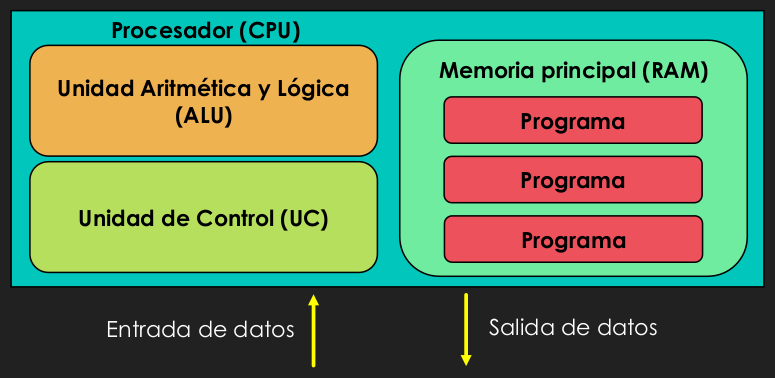
\includegraphics[scale=0.5]{estructura-ordenador1.png}
\caption{Diagrama de un ordenador}
\label{fig:c1fig1}
\end{figure}

\begin{figure}[h]
\centering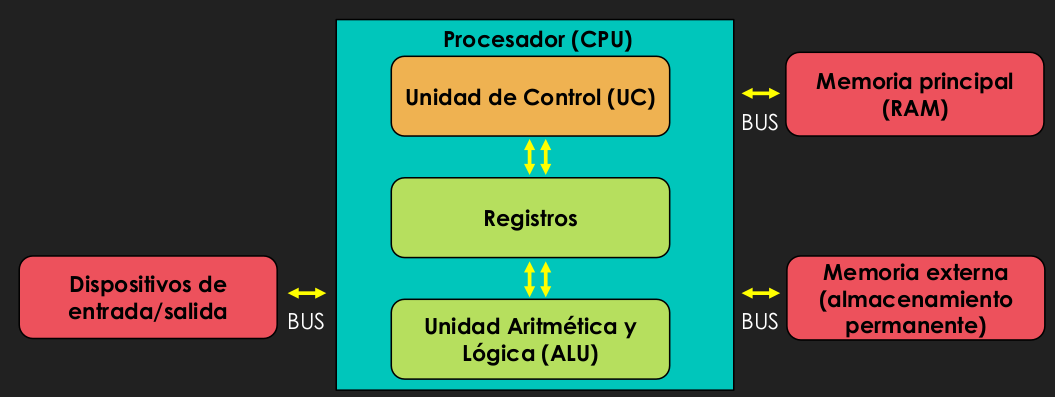
\includegraphics[scale=0.4]{estructura-ordenador2.png}
\caption{Esquema de la CPU y los buses del sistema}
\label{fig:c1fig2} 
\end{figure}

\begin{table}[h]
\centering
\begin{tabular}{l l l}
\toprule
\textbf{Unidad} & \textbf{Equivalencia}\\
\midrule
Byte (B) & 8 bits \\
Kilobyte (KB) & 1024 bytes \\
Megabyte (MB) & 1024 Kbytes \\
Gigabyte (GB) & 1024 Mbytes \\
Terabyte (TB) & 1024 Gbytes \\
Petabyte (PB) & 1024 Tbytes \\
\bottomrule
\end{tabular}
\caption{Unidades de medida de almacenamiento}
\label{tab:c1tab1} 
\end{table}

1 TB = 1024 GB = 1024 x 1024 Mb = 1.048.576 KB = 1.073.741.824 Bytes

\section{Representación de la información}



\section{Ejercicios propuestos}

Completa tu aprendizaje realizando los siguientes ejercicios propuestos:

 % Se incluye el capítulo 3

%----------------------------------------------------------------------------------------
%	CAPÍTULO 4
%----------------------------------------------------------------------------------------
%----------------------------------------------------------------------------------------
%	CAPÍTULO 4
%----------------------------------------------------------------------------------------
\chapterimage{chapter_head_2.pdf} % Imagen del capítulo

\chapter{¿Qué es un algoritmo?}

\section{Concepto de algoritmo}

\section{Características de un algoritmo}

\section{Resolución de problemas}

\section{Creación de algoritmos}

\subsection{Pseudocódigo}

\subsection{Representación gráfica}

\section{Paradigmas de programación}

\section{Lecturas recomendadas}

\section{Software y tipos de software}

\section{Lenguajes de programación}

\section{Ejercicios propuestos}

Completa tu aprendizaje realizando los siguientes ejercicios propuestos:

\begin{exercise}
Bla bla bla
\end{exercise}

\begin{exercise}
Bla bla bla
\end{exercise}

\begin{exercise}
Bla bla bla
\end{exercise}

\begin{exercise}
Bla bla bla
\end{exercise}
 % Se incluye el capítulo 4
 % Se incluye la parte I

%----------------------------------------------------------------------------------------
%	PARTE II
%----------------------------------------------------------------------------------------
\part{Programación en C/C++}
 % Se incluye la parte II

%----------------------------------------------------------------------------------------
%	PARTE III
%----------------------------------------------------------------------------------------
\part{POO en Java}
 % Se incluye la parte III

%----------------------------------------------------------------------------------------
%	BIBLIOGRAFÍA
%----------------------------------------------------------------------------------------

\part*{Bibliografia e índice alfabético}

\chapter*{Bibliografía}
\addcontentsline{toc}{chapter}{\textcolor{ocre}{Bibliografía}} % Se añade el encabezado de la bibliografía en el índice de contenidos
 
%------------------------------------------------

\section*{Libros de referencia}
\addcontentsline{toc}{section}{Libros de referencia}
\printbibliography[heading=bibempty,type=book]

%----------------------------------------------------------------------------------------
%	ÍNDICE
%----------------------------------------------------------------------------------------

\cleardoublepage % Nos aseguramos que el índice empiece en una página impar (lado derecho)
\phantomsection
\setlength{\columnsep}{0.75cm} % Fija el espaciado entre las dos columnas del índice
\addcontentsline{toc}{chapter}{\textcolor{ocre}{Índice alfabético}} % Añade el encabezado del índice en el índice de contenidos
\printindex % Imprime el índice

%----------------------------------------------------------------------------------------

\end{document}
